\chapter{Google Protocol Buffers}
\label{cha:appendixA}
W tym dodatku zostanie omówiona idea oraz szczegóły implementacyjne stojące za Google Protocol Buffers, dalej zwanym \textit{ProtoBuf}.
Omówione zostaną również przykładowe zastosowania, oraz dlaczego warto porzucić w niektórych sytuacjach komunikację przy pomocy
XML bądź JSON, na rzecz Protocol Buffers lub mu podobnym binarnym protokołom komunikacji.

%---------------------------------------------------------------------------
\section{Zasada działania}
\label{sec:protobuf_history}

Protocol Buffers powstało pierwotnie jako wewnętrzny projekt Google, mające na celu zmniejszenie ilości ruchu
na łączach oraz zwiększenia szybkości z jaką wiadomości wysyłane między serwerami są serializowane oraz deserializowane.
W momencie pisania wewnątrz Google znajduje się 48,162 typów wiadomości, rozproszonych w 12,183 plikach -- są to imponujące liczby,
obrazujące jak ważnym elementem infrastruktury Google stał się ProtoBuf. \cite{protobuf}

Protocol Buffers, dalej zwane ProtoBuf, opierają się w dużej mierze o język definicji interfejsu (\textit{IDL}) o tej samej nazwie.
Przy jego pomocy definiuje się tak zwane wiadomości, które mogą zawierać pola lub zagnieżdżone wiadomości i/lub enumeracje.
Tak przygotowany opis wiadomości, zapisany w tak zwanym proto-pliku (,,\textit{proto-file}'') następnie poddawany jest kompilacji,
przy pomocy narzędzia \textit{protoc} (\textit{Proto}col Buffers \textit{C}ompiler) czego wynikiem są klasy (o ile taka abstrakcja jest dostępna
w wybranym języku docelowym) które udostępniają bezpieczne (co do typów) API do manipulacji tymi wiadomościami oraz, co ważniejsze, 
,,potrafią się same przeczytać z strumienia bajtów''. Pod tym zwrotem kryje się zwyczajna implementacja fabryki, potrafiąca dekodować 
strumień bajtów zakodowany dla pewnej wiadomości, do postaci obiektu danej klasy.

\newpage
Jako przykład możemy spojrzeć na poniższą deklarację wiadomości (Listing \ref{proto_simple_sam}):
\begin{lstlisting}[label={proto_simple_sam}]
message Person {
  required string name = 1;
  optional string email = 3;
  message PhoneNumber {
    required string number = 1;
    optional PhoneType type = 2 [default = HOME];
  }
  repeated PhoneNumber phone = 4;
}
\end{lstlisting}

Który po skompilowaniu do języka \textit{C++}, wygenerowałby klasę potrafiącą obsłużyć następujące operacje:

\begin{lstlisting}[caption={Przykład klasy ProtoBuf w C++, pisanej na plik}]
Person person;
person.set_name("John Doe");
person.set_id(1234);
person.set_email("jdoe@example.com");
fstream output("myfile", ios::out | ios::binary);
person.SerializeToOstream(&output);
\end{lstlisting}

A następnie możliwe byłoby dokonanie opisywanej wcześniej deserializacji z utworzonej właśnie tablicy bajtów:

\begin{lstlisting}[caption={Przykład klasy ProtoBuf w C++, odczytującej ,,się'' z zapisanego wcześniej binarnego pliku}]
fstream input("myfile", ios::in | ios::binary);
Person person;
person.ParseFromIstream(&input);
cout << "Name: " << person.name() << endl;
cout << "E-mail: " << person.email() << endl;
\end{lstlisting}

Analogicznie wynegerowane klasy można otrzymać w praktycznie dowolnym języku programowania, 
przy czym wspieranymi przez Google językami są C++, Java oraz Python. Do generowania klas dla pozostałych języków
służą implementowane przez społeczność open source pluginy do kompilatora protoc.

Łatwo jest sobie wyobrazić powyższy przykład, piszący zamiast do pliku, na strumień będący odbieranym przez klienta po drugiej stronie.
Tak właśnie w dużym przybliżeniu implementowane są web serwisy przy wykorzystaniu Protocol Buffers. Istnieją dodatkowe pomocnicze fabryki oraz metody
korzystania z ProtoBuf jako zasobów sieciowych, na przykład implementacje Protocol Buffers w oparciu o standard JAX-RS \cite{jaxrs}.


%---------------------------------------------------------------------------
\section{Wyjaśnienie znaczenia pól Protocol Buffers}
\label{sec:typeQialifiers}

\begin{lstlisting}[caption={Przypomnienie wyglądu deklaracji pola wiadomości}]
 required string name = 45 [ default = "sample" ];
\end{lstlisting}

W przedstawionej w 1 sekcji tego rozdziału wiadomości (Listing \ref{proto_simple_sam}) można zauważyć iż każde pole składa się z następujących elementów:

\begin{itemize}
 \item \textbf{Kwalifikatora}, który może przyjąć wartości:
  \subitem \textbf{required} - oznaczającym że pole \textit{musi} zostać ustawione. Generalnie odradza się jego stosowania, ponieważ 
                               pole raz oznaczone tym kwalifikatorem, musi zawsze pozostać required. Nawet jeżeli przestanie być kiedyś w przyszłości używane.
  \subitem \textbf{optional} - oznaczającym że pole może ale nie musi zostać ustawione. Jest to zalecany kwalifikator w większości przypadków.
  \subitem \textbf{repeated} - oznaczającym listę. Pole oznaczone tym kwalifikatorem może powtarzać się dowolną ilość razy w wiadomości.
 \item \textbf{Typu pola} - mogącym być jednym z predefiniowanych w Protocol Buffers typów (wylistowanych w Tabeli \ref{protoYypes_all}, lub typem wiadomości lub enumeracji
                            zdefiniowanym przez użytkownika.
 \item \textbf{Nazwy pola} - nazwa pola, poprawne indentyfikatory są zgodne z standardem stosowanym przez Javę
 \item \textbf{TAG}u - tag jest specjalną liczbą, nie mogącą powtarzać się w obrębie jednej wiadomości. Liczba ta jest wykorzystywana podczas kodowania 
                       wiadomości do jej możliwie najoptymalniejszej postaci. Warto pamiętać że umieszczenie często używanych pól jako pierwszych \textit{ma wpływ}
                       na ostateczny rozmiar wiadomości. Ponieważ w przypadku pól o wysokich tagach, które rzadko, lub nigdy nie są ustawiane, nie zostaną one w ogóle 
                       umieszczone w zserializowanej postaci wiadomości - oszczędzając cenne bajty.
 \item \textbf{default} - wartość domyślna \textit{nie jest konieczna} jednak możliwa do podania przy każdym polu -- sens ma oczywiście jednak tylko w przypadku 
                          podania jej dla pola będącego typu \textbf{optional}, ponieważ w przypadku \textbf{required} wartość ta i tak zostałaby nadpisana.
                          W przypadku pola typu enumeracyjnego, możliwe jest podanie stałej z wewnątrz tej enumeracji jako wartości domyślnej.
\end{itemize}

\begin{table}
\begin{center}
\begin{tabular}{llll}
sint32 & bytes & double & uint64\\
sint64 & string & float & uint32\\
fixed32 & bool & int32 & int64 \\
sfixed32 & sfixed64 & fixed64 &  \\
\end{tabular}
\end{center}
\label{protoTupes_all}
\caption{Predefiniowane typy w ProtoBuf}
\end{table}

Poza wspomnianymi predefiniowanymi typami, pola mogą oczywiście mieć typ innej wiadomości. Tym sposobem można modelować nawet skomplikowane modele domenowe
w obrębie wiadomości ProtoBuf. Innym typem który mogą przyjąć pola, są type enumeracyjne. Deklaruje się je w podobny sposób jak wiadomości, jednak 
ich pola mają mniej elementów koniecznych do podania. Przykład deklaracji enumeracji można zobaczć na Listingu \ref{lst:enumDeclaration}.

\begin{lstlisting}[caption={Deklaracja oraz zastosowanie typu enumeracyjnego}, label={lst:enumDeclaration}]
enum TheEnum {
  SMALL = 1;
  LARGE = 2;
}

message It {
  optional TheEnum itsName = 1 [ default = LARGE ]
}
\end{lstlisting}

Jak widać, możliwe jest również podanie nazwy \verb|LARGE| jako wartości domyślnej pola.


%---------------------------------------------------------------------------
\section{Zestawienie wydajności mechanizmów serializacji na JVM}
\label{sec:serialization_speed}

Poniewać w efekcie, ProtoBuf służy efektywnej serializacji i deserializacji obiektów, bardzo ważna jest jego wydajność na realnych obiektach.
Testy takie przeprowadzono w ramach projektu umieszczonego na githubie pod adresem: \href{https://github.com/eishay/jvm-serializers/wiki/}{https://github.com/eishay/jvm-serializers/wiki/}.
Benchmark \cite{proto_benchmark} ten został wykonany w roku 2011, oraz uwzględnia najważniejsze metody serializacji danych na JVMie, takie jak
natywna serializacja Java, serializacja danych do JSON przy pomocy różnych bibliotek oraz oczywiście ProtoBuf oraz jego konkurencji - Thrift.

\textbf{Serializacja + Deserializacja:}\\
Czas spędzony na serializacji oraz deserializacji tego samego obiektu:

\begin{figure}[ch!]
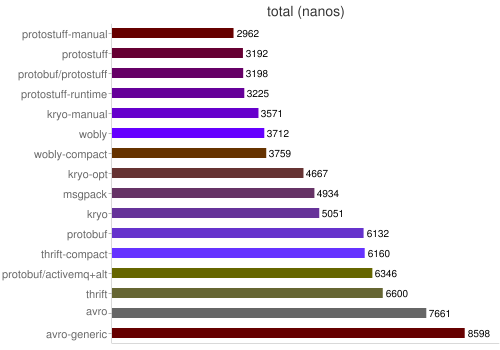
\includegraphics[width=\textwidth]{proto_1}
% 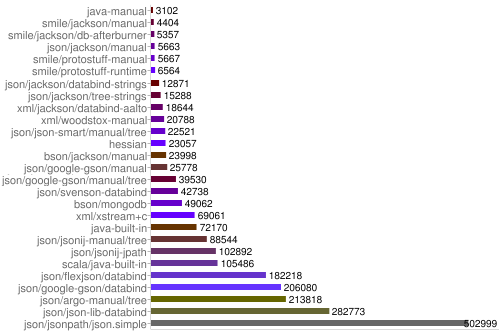
\includegraphics[width=\textwidth]{proto_2} TODO TODO TODO
\end{figure}

ProtoStuff, alternatywna implementacja protokołu ProtoBuf wiedzie prym w tym benchmarku, jednak protobuf nadal jest stanowczno wiadącą implementacją.
Najważniejszą obserwacją tutaj jest jednak porównanie binarnych protokołów, które zmieściły się na powyższym wykresie, do metod serializacji JSONowej.
Dla przykłądu Google Gson, jedna z popularniejszych bibliotek serializacji Java -> JSON, tą samą serializację przeprowadziła w \textbf{25778ns}, co w porównaniu
z czasem osiągniętym przez ProtoBuf, równym \textbf{6132ns} jasno wyraża przewagę z jaką ProtoBuf wyprzedza serializację ,,klasyczną''.

\newpage
\textbf{Rozmiar zserializowanej wiadomości:}\\
Rozmiar liczony w bajtach wiadomości po zserializowaniu:

\begin{figure}[ch!]
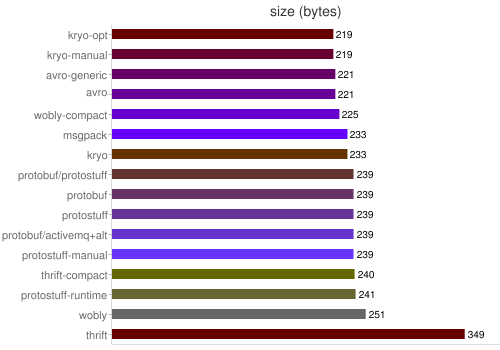
\includegraphics[width=\textwidth]{serialized_size_1}
% 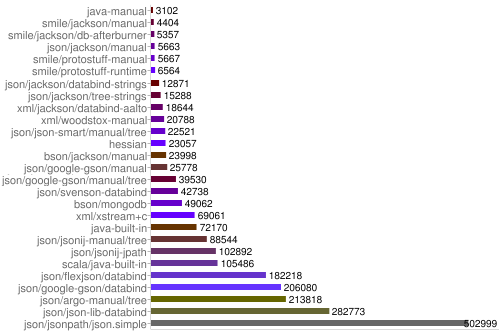
\includegraphics[width=\textwidth]{proto_2} TODO TODO TODO
\end{figure}

Przy porównywaniu rozmiaru zserializowanego obiektu ponownie protokoły binarne, z ProtoBuf na czele wiodą prym... 
Konkurencja typu serializacji Javowej lub JSON niestety nie ma tutaj wiele do powiedzenia, powodem jest iż Java serializując obiektu musi
zatrzymać wszystkie nazwy klas aby potrafić się do nich odwołać podczas deserializacji; W przypadku JSONa, mamy do czynienia z dużą ilością nadmiarowych danych
w postaci reprezentowania liczb jako tekst, oraz dużej ilości nadmiarowych znaków w postaci \verb|{| oraz \verb|}| itp.



%---------------------------------------------------------------------------
\newpage
\section{Przykładowe definicje wiadomości}
\label{sec:proto_file_examples}

Poniżej zostanie przedstawione kilka przykładowych definicji wiadomości, celem zapoznania czytelnika z formatem i składnią protobuf w
sposób bardziej praktyczny (wizualny).

\begin{lstlisting}[caption={Definicja wiadomości zawierająca enum oraz wartości domyślne}]
message SearchRequest {
  required string query = 1;
  optional int32 page_number = 2;
  optional int32 result_per_page = 3 [default = 10];

  enum Corpus {
    UNIVERSAL = 0;
    WEB = 1;
    IMAGES = 2;
    LOCAL = 3;
    NEWS = 4;
    PRODUCTS = 5;
    VIDEO = 6;
  }

  optional Corpus corpus = 4 [default = UNIVERSAL];
}
\end{lstlisting}

\begin{lstlisting}[caption={Definicja wiadoomści wykorzystującej inną wiadomość}]
message SearchResponse {
  repeated Result result = 1;
}

message Result {
  required string url = 1;
  optional string title = 2;
  repeated string snippets = 3;
}
\end{lstlisting}

\newpage
\begin{lstlisting}[caption={Definicja wiadomości korzystającej z wewnętrznej wiadomości}]
package pl.project13.protodoc;

message SearchResponse {
  message Result {
    required string url = 1;
    optional string title = 2;
    repeated string snippets = 3;
  }
  repeated Result result = 1;
}
\end{lstlisting}

Więcej przykładów można zobaczyć na stronie domowej Protocol Buffers - \href{http://code.google.com/intl/pl-PL/apis/protocolbuffers/docs/proto.html}{http://code.google.com/intl/pl-PL/apis/protocolbuffers/docs/proto.html}.
Niestety podczas realizacji projektu nie udało się pokryć pełnego formatu protocol buffers, jest to jednak logiczny kierunek dalszego rozwoju aplikacji.
